\documentclass[UTF8]{article}

%--
\usepackage[UTF8]{ctex}
\usepackage[margin=1in]{geometry}
\usepackage{graphicx}
\usepackage{caption2}
\usepackage{subfigure}
\usepackage{float}

%--
\begin{document}
    
%--
%{\flushleft \bf \Large 姓名:} 汪清悦
%
%{\flushleft \bf \Large 学号:} MG1933055
%
%{\flushleft \bf \Large 日期:} 2019.11.10


%=========================================================================
\section*{论文信息}
    
本次报告主要围绕一致性算法展开,介绍两种受欢迎的一致性算法——Paxos和Raft,并将这两种“风格迥异”的一致性算法进行对比。参考的论文主要包括:

%--    
\begin{itemize}
    \item Lamport, L. \emph{Paxos made simple}. ACM SIGACT News 32, 4 (Dec. 2001), 18–25
    \item Diego Ongaro and John Ousterhout, Stanford University. \emph{In Search of an Understandable Consensus Algorithm}. USENIX 2014 (best paper)
\end{itemize}

本次报告的结构如下:
\begin{list}{~}{~}
	\item 第一章:介绍分布式系统中的一致性问题,阐述一致性算法要解决的问题。
	\item 第二章:详细介绍一致性算法的鼻祖——Paxos,包括个人角度理解的Paxos一致性保证的讨论。
	\item 第三章:详细介绍更“年轻”、更容易理解的Raft一致性算法,主要包括Leader selection 和 Log replication 过程,以及其日志一致性的讨论。
	\item 第四章:对比Raft相比于Paxos的异同。
\end{list}
    
%请严格按照课程PPT上的要求,来选取报告所讨论的文献。
%    
%参见“https://github.com/alg-nju/intro-disalg-course/blob/master/further-reading.md”上提供的基本文献。其它文献参见课程PPT上的描述。
%
%如果希望讨论一篇上面没有提及的文献,欢迎提前跟老师当面沟通。在得到老师的认可之后,方可按自己选的文献完成报告。


    
%=========================================================================
\section{一致性问题}

%论文信息之后,是半开放的讨论。可以根据讨论的内容,自己拟订不同章节的名字。
%
%课上会做一个较为详细的解释。
%
%常见的内容包括:
%
%%--    
%\begin{itemize}
%    \item 基本模型、基本假设:分布式系统的基本模型往往比较复杂。实际论文中的模型与课本中的模型比,要精细地多。大家需要按照课上讲的框架,把论文中模型的各个纬度都讨论清楚。
%    
%    \item 基本问题:是否是经典问题。即使对于经典问题(e.g. consensus),也有很多的变体。把问题全面认识清楚,与解决问题一样重要。对于一些不经典的问题,可以参照课上的学习,将问题全面地认识清楚,解释清楚。
%    
%    \item 主要贡献:对于论文贡献的深入解释,往往是一个具体的模型、算法、分析技术。技术的细节不是最重要的,简单copy原文更是大忌。课程看重的是,从课程中所学习的视角进行分析解读,进行原理性的提炼、阐述等。另外,虽然我们是偏理论的课程,但是对于实现、实验、系统的解读也是欢迎的,例如,系统设计、实现的背后,理论建模与分析是如何发挥指导性作用的,等等。
%    
%    
%上诉内容,如有疑问,欢迎跟老师讨论。
%     
%\end{itemize}

一致性算法用来解决一致性问题,而一致性问题是分布式系统中的经典问题。

为了解决单机操作系统计算及存储资源的不足,分布式系统应运而生。为了避免单点故障,数据在分布式系统中通常有多个备份,这使得分布式集群有更好的错误容忍度。
一致性问题是指对于一组服务器,给定一组操作,我们需要一个协议(一致性算法)使得最后它们的结果达成一致。
更详细地说,当其中某个服务器收到客户端的一组指令时,它必须与其它服务器交流以保证所有的服务器都是以同样的顺序收到同样的指令,这样,所有的服务器会产生一致的结果,看起来就像是一台机器一样。


%=========================================================================
\section{Paxos}

Paxos算法是Lamport于1990年提出的一种基于消息传递(不考虑Byzantine事件)且具有高度容错特性的一致性算法。

起初,Lamport用Greek的例子来描述这个算法的主要思想,但实在难以理解;之后,Lamport用英文描述了Paxos算法,虽然可读性提高,但是Paxos算法本身还是十分复杂,需要阅读更多的资料才能够基本理解Paxos。这也正是之后的一些更易理解的一致性算法出现的初衷。

Paxos算法解决的问题是一个分布式系统如何就某个值(决议)达成一致。它实际上是一个共识算法。

\subsection{问题描述}

设想一组可以提出提议的process。一致性算法保证所有提出的提议中,只有一个提议会被选择。如果没有提出提议,那么将不会有提议被选择。如果一个提议被选择,那么所有process可以学习到这个提议。一致性算法需要的安全性要求是:
\begin{enumerate}
	\item 仅可以选择被提出的提议
	\item 仅有一个提议会被选择
	\item process不会知晓一个值被选择了,直到这个值确实被选择了
\end{enumerate}

\subsection{Paxos 一致性算法}

Paxos算法中划分了3个角色:proposer(提出者)、acceptor(批准者)和learner(学习者)。一个process可以扮演多个角色,并假设process之间的通信是基于消息的、异步的、非Byzantine模型的。

每个提议有一个为实数的编号n以及提议内容v,因为一个提议用\{n, v\}表示,其中n全序且唯一的。

\subsubsection{达成一致的过程}

\paragraph{两个阶段}
选择唯一的提议的过程分为两个阶段:

\begin{itemize}
	\item 阶段一:Prepare
		\begin{enumerate}
			\item Proposer:选择一个提议,编号为n,向acceptor的多数派发送编号为n的prepare请求。
			\item Acceptor:如果接收到的prepare请求的编号n大于它已经回应的任何prepare请求,它就回应此请求。Acceptor将告知已经接受的编号最高的提议的内容,并承诺不再回应任何编号小于n的提议。
		\end{enumerate}
	\item 阶段二:Accept
		\begin{enumerate}
			\item Proposer:如果收到了多数acceptor对prepare请求(编号为n)的回应,它就向这些acceptor发送提议\{n, v\}的accept请求,其中v是所有acceptor回应中编号最高的提议的内容(如果收到的所有acceptor的回应都不带有其已经接受的提议,说明当前提议将是这些acceptor收到的第一个提议,这时,提议的内容可以是任意的)。
			\item Acceptor:当收到提议\{n, v\},如果此acceptor在此期间没有接受过任何编号大于n的提案,则接受此提案内容,否则忽略。
		\end{enumerate}
\end{itemize}

\paragraph{一致性保证}

在Paxos论文中,包含关于以上算法的一致性的论证。以下就我个人角度及观点,讨论以下两个Paxos的一致性要求:

\begin{enumerate}
	\item Acceptor必须接受它接收到的第一个提议。
	\item 如果一个提议\{n, v\}被选择/接受,那么每一个编号更高的被选择的提议包含的值都是v。
\end{enumerate}

第一个要求是显而易见的,在没有消息丢失等异常的情况下,即使仅有一个proposer提出了一个提议,我们也希望acceptor能够接受这个提议。因此,acceptor应该接受它接收到的第一个提议(对应到Paxos的Accept阶段,acceptor接受收到的第一个Accept请求)。

Paxos的Prepare阶段保证了第二个要求,它使得:如果一个提议\{n, v\}被选择,那么每一个acceptor接受的编号更高的提议包含的值都是v。这是通过acceptor在prepare阶段对proposer的回应保证的,prepare阶段能够保证:如果一个提议\{n, v\}已经被返回prepare回应的acceptor选择,那么此后,任何proposer提出的编号更高提议包含的值都是v。

结合这两个要求,我们可以通过简单的类似第二数学归纳法的思想来证明一致性。就我个人的理解,在这个问题中,要求一找到了第一个被接受的提议,相当于保证了“最小数”依据的存在;要求二保证了后续的提议相对于之前的提议来说都是可归纳的。从而Paxos能够保证一致性过程结束后能够达到最终一致性。

\subsubsection{处理流程}

\paragraph{Learner获知已经被选择的值}

达成一致性的过程是proposer和acceptor两个角色之间的交互,learner角色需要在达到一致之后获得一致的结果。

最简单的方法是,让每个acceptor在批准提议的时候通知所有的learner,把批准的提议发给learner。但一个显而易见的问题是,告知learner所需的消息数量(learner数与acceptor数的乘积)过于庞大。

另一种方法是,让acceptor将接受情况回应给一个主learner,它再把被选择的值通知给其它的learner。这增加了一次额外的消息传递,会比前一种不可靠一些,因为主learner可能会失效,但是这个方法要求的消息个数仅是learner数和acceptor数的总和。

更一般的,acceptors可以通知多个主learners,每个主learner都能通知其它所有的learners。主learner越多越可靠,但是通信复杂性会增加。

\paragraph{为了确保达到一致过程能够结束,引入主proposer}
Paxos选择唯一的提议的过程确实能够保证一致性,但这个达到最终一致性的过程对应到实际的处理流程时依旧存在问题。

设想这样一个场景,两个proposer轮流提出一系列编号递增的议案,但是都没有被选择。Proposer p用提议的编号为n1,并结束阶段1;另外一个proposer q选择了提议编号n2 > n1,并结束阶段1。于是p在阶段2的accept请求将被忽略,因为acceptor已经承诺不再批准编号小于n2的议案。于是p再回到阶段1并选择了编号n3 > n2,这又导致q第二阶段的accept请求被忽略;这样一直循环下去……

为了避免这种情况(即保证达到最终一致的过程能够结束),Paxos规定必须选择一个主proposer——只有主proposer才能提出提议。如果主proposer和多数acceptor成功通信,并提出一个编号更高的提议,提议将被接受,值会被选择。如果它得知已经有编号更高的议案,它将放弃当前的提议,主proposer最终能选择一个足够大的编号。

Paxos并未对主proposer的选择做规定,但Paxos指出选择主proposer的可靠算法必须使用随机或者实时——例如,使用超时机制。

\subsubsection{实现}

Paxos算法假设了一个某些process组成的网络。在其一致性算法中,每个process都同时扮演proposer、acceptor和learner的角色。算法选择一个leader,它就是主proposer和主learner。在考虑实现时,需要使用持久化存储来保证acceptor失效后也能记住必要的信息,acceptor在发送响应前必须持久化存储该响应。

此外,需要一个保证任何两个提议的编号都不相同的机制。Proposer从互不相交的集合中选择议案编号,因此两个不同的proposer永远不会提出相同编号的议案。每个proposer都持久化保存它已经提出的编号最高的提议,并使用一个更高的提议编号来开始Prepare阶段。

%=========================================================================

\section{Raft}

Paxos是分布式系统中最早的一致性算法,它与“更年轻的”Raft算法都是目前最受欢迎的一致性算法。相比于Paxos,Raft更加容易理解。在Raft中,server之间是基于消息(RPC)通信的。与Paxos不同,它将一致性的过程分为 Leader Election 和 Log Replication 两个部分。

\paragraph{服务器状态}

在任何一个时刻,Raft集群中的 server 处于Leader、Follower或者Candidate三种状态之一。Candidate状态的 server 只会出现在Leader election阶段。在正常操作过程只有一个 server 作为Leader,其他 server 作为Follower被动地处理来自Candidate和Leader的请求。图\ref{fig:raft_state}是三个状态之间的转换,我将在后面的章节中详细描述。

\begin{figure}[h]
	\centering
	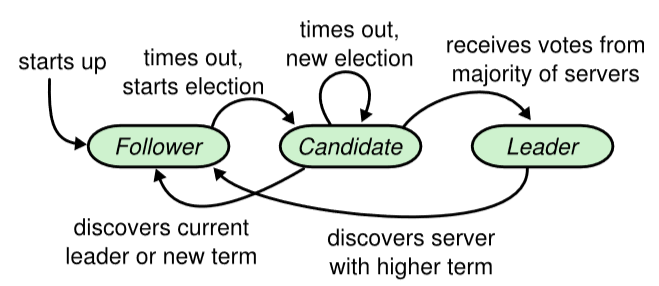
\includegraphics[width=0.7\linewidth]{figures/raft_state}
	\caption{Raft server状态转化}
	\label{fig:raft_state}
\end{figure}


\paragraph{任期}

Raft 将时间分为多个连续的任期term,如图\ref{fig:raft_term}所示,每个任期从 Leader election 阶段开始。Leader election 结束后选举出唯一的 server 作为这个任期的Leader,Leader周期性地向所有Follower发送 heartbeat来宣告自己能够胜任Leader;Leader election 也可能会出现选票瓜分从而无法选出唯一的Leader的情况,这时直接结束这个任期,开始下个任期。因此,Raft确保了每个任期最多只有一个Leader。

\begin{figure}[h]
	\centering
	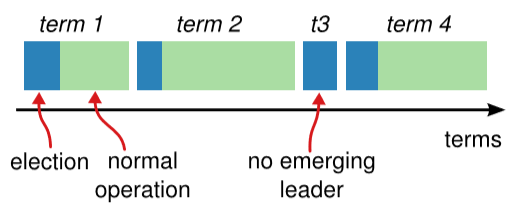
\includegraphics[width=0.5\linewidth]{figures/raft_term}
	\caption{Raft任期}
	\label{fig:raft_term}
\end{figure}

\subsection{Leader Election}\label{section:raft_leaderElectione}

Learn Election过程用来选出最多一个server作为任期的Leader。

\subsubsection{具体过程}

Raft通过heartbeat机制来触发Leader election。初始时,所有 server 都是Follower状态。

\paragraph{Follower}

\begin{itemize}
	\item 回应来自Candidate和Leader的请求。
	\item 如果Follower在election timeout内没有收到 heartbeat消息,它会认为Leader这时候可能发生了故障,从而开始一个 Leader election 阶段来选出新的Leader。注意,election timeout 取150-300ms之间的随机值,从而极大程度地减少了选票瓜分情况发生的概率。
		\subitem 在 Leader election开始时,Follower更新任期并转变为Candidate。
\end{itemize}

\paragraph{Candidate}

\begin{itemize}
	\item 转变为Candidate后:
		\subitem 更新任期
		\subitem 重置election timer
		\subitem 向集群中的其他 server 分发选票
	\item 如果收到了大多数 server 的选票,则胜出,成为这个任期的Leader。
	\item 如果收到了heartbeat消息:
		\subitem heartbeat消息中夹带的任期信息没有过期,则已经选出Leader,它将转变为Follower。
		\subitem heartbeat消息中夹带的任期信息已过期,继续Candidate状态。
	\item 如果在一段时间内没有出现以上两种情况,说明可能有多个Follower同时转变为Candidate状态,并将选票瓜分了,从而没有一个Candidate能够收到足够的选票从而成为Leader。此时,Candidate触发超时,结束这个任期,开始新一任期的 Leader election。
\end{itemize}

\paragraph{Leader}

从Candidate转变为Leader后,它向其他所有 server 周期性地发送 heartbeat 消息来宣告自己是这个任期内的Leader并ni正常运作(防止Follower触发election timeout)。

\subsection{Log Replication}

\subsubsection{日志组织结构}

Raft的日志组织结构如图\ref{fig:raft_log}所示。每个日志条目存储一条状态机指令和领导人收到该指令时的任期号(任期号用于检测多个日志副本之间不一致的情况)。为了保证日志匹配的原则,每个条目都有一个整数索引来表示它在日志中的位置。

\begin{figure}[h]
	\centering
	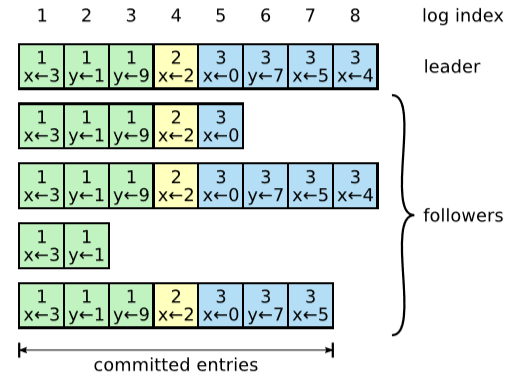
\includegraphics[width=0.5\linewidth]{figures/raft_log}
	\caption{Raft的日志结构}
	\label{fig:raft_log}
\end{figure}

\subsubsection{具体过程}

\paragraph{Leader} 在Leader Election成功选出Leader之后,Leader就开始接收Client请求。

\begin{itemize}
	\item Leader收到Client的请求,生成对应的日志条目,并把生成日志条目的请求并行地广播给所有的Follower。
	\item 如果超过一半的Follower都返回success,Leader会认为这个条目是可提交的,Leader就会正式执行这个日志条目,并将执行结果返回给Client。 
\end{itemize}

\paragraph{Follower}

每个Follower在收到Leader的请求后有两种选择:
\begin{itemize}
	\item 听从Leader的请求,写入日志条目并返回success。
	\item 在某些条件不满足的情况下,Follower无法写入日志条目,返回false。
\end{itemize}

另外,在Raft算法中,Leader通过强制Follower复制它的日志来处理日志的不一致。这就意味着,在Follower上的冲突日志会被Leader的日志覆盖掉。

\subsubsection{日志的一致性讨论}

Raft中日志的一致性主要基于Raft的日志机制能够满足以下两个特性: 
\begin{itemize}
	\item 如果在不同的日志中的两个条目拥有相同的索引和任期号,那么他们存储了相同的指令。
	这是因为,Leader在一个任期里在给定的日志索引位置最多创建1条日志条目,同时该条目在日志中的位置也不会改变。
	\item 如果在不同的日志中的两个条目拥有相同的索引和任期号,那么他们之前所有的日志条目也全部相同。
	这个特性源于heartbeat的一个简单的一致性检查。当发送一个heartbeat时,Leader会把新的日志条目紧接着的之前的条目的索引位置和任期号都包含在里面 。如果Follower没有在它的日志中找到相同索引和任期号的日志,它就会拒绝新的日志条目。这个一致性检查就像一个归纳的步骤,只要heartbeat返回成功的时候,Leader就知道Follower的日志和它的是一致的。
\end{itemize}

%=========================================================================
\section{对比Raft与Paxos}

通过以上对Paxos和Raft的描述,应该能够很直观地感受到Paxos一致性算法本身是有些复杂并且难以推理的,而Raft算法十分清晰,并且易于实施。因此,研究人员通常对Paxos更感兴趣,但Raft更受到工程师的欢迎。Raft与Paxos的“年纪”相差二十年有余,Raft在为一致性算法注入新鲜血液的同时也与Paxos算法有一些相同之处。

\paragraph{服务器——确定状态机} 两者在涉及到实现时,都将server看作是确定状态机(Raft沿用了Paxos),一致性过程保证了每台状态机执行相同的指令从而得到最终的一致性结果。

\paragraph{唯一Leader} Paxos和Raft在正常操作期间都有唯一一个Leader来协调系统的一致性。唯一的Leader协调系统中所有server的状态,使得一致性算法更容易规定和实施。同时,这个唯一的Leader也可能成为系统的性能瓶颈。

\paragraph{Leader Election}Raft中明确规定了Leader Election过程,在这个过程中也暗示了Raft中只有拥有最新信息的server才会成为Leader;而Paxos中没有定义如何推举出Leader,任何一个server都可能成为Leader。

\paragraph{决策方案} Paxos和Raft所遵循的决策方案本质上是相同的——多数同意即可(Raft沿用了Paxos)。

\paragraph{活跃度} 两种算法的决策方案决定了它们都可以保证:只要大多数server还正常工作,就能正常提供服务。

    
%--
\end{document}